\include{tex/headerueb}
\include{tex/header}
\include{tex/info}

\newcommand{\nr}{6}
\lstset{language=matlab}

\begin{document}
\section*{Aufgabe 1 - Histogram-Abstand}
Zur Berechnung der Histogrammen konnten die Funktionen aus Zettel 6 wiederverwendendet werden.
Abbildung \ref{hist} zeigt die V-Histogramme der Banenenbilder und als Vergleich das Histogramm von Lenna (gepunktet).

\begin{figure}[H]
\begin{center}
\includegraphics[width=100mm]{u09/hist.eps}
\end{center}
\label{hist}
\caption{Histogramme der Bilder}
\end{figure}

Die Abstandsmasse wurden wie in der Vorlesung gezeigt implementerit und die Abstaende zwischen den Bildern einzelnd fuer U und V Kanal bestimmt.
Abbildung \ref{dist} zeigt die Abstatende der Histogramme. Da KL-Divergenz nicht symetrisch ist, sind beide Ergenisse in der Tabelle dargestellt.
Sowohl bei Euklid sowie bei KL ist die Naehe der Bannenen-Bilder im vergleich zu Lenna deutlich zu sehen.
Da die KL-Divergenz grosse Unterschiede bei Vertauschung der Argumente aufweist, waere es fuhr den einsatz wohl sinnvoll einen Mittelwert zu bilden.

\begin{figure}[H]
\begin{center}
\begin{tabular}[h]{|l|ll|ll|}
\hline
                & \multicolumn{2}{c|}{Euklidisch} & \multicolumn{2}{c|}{KL-Divergenz} \\
Bilder          & U & V & U & V \\
\hline
Banana 1 \& 2   & 0.047815 & 0.11121 & 0.043122 & 0.28096 \\
                &          &         & 0.11906  & 0.20736 \\
Lenna vs Banana & 0.23289  & 0.35372 & 0.94327  & 0.80404 \\
                &          &         & 0.26069  & 3.2175  \\
\hline
\end{tabular}
\end{center}
\label{dist}
\caption{Ergebnisse}
\end{figure}

\section*{Aufgabe 2 - HOP}

Mit dem Soebel-Operator aus vorherigen Zetteln wird die Ableitung der Bilder bestimmt. 
In $32\times 32$ Zellen unterteild werden die Vektoren der Abschnitte aufsummiert und anschliessend der Winkel der Summenvectoren bestimmt.
Abbildung \ref{theta} zeigt die Winkel der Zellen. Um Vergleichswerte zu gennerieren wird wieder Lenna mit den Bananen verglichen.

\begin{figure}[H]
\begin{center}
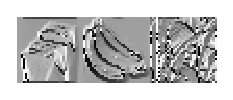
\includegraphics[width=100mm]{u09/the.eps}
\end{center}
\label{theta}
\caption{Winkel der Zellen}
\end{figure}

Schliesslich werden die Histokgramme der Winkel besimmt. In Abbildung \ref{thist} ist deutlich zu erkennen, 
dass die Bannenen-Bilder deutlicher, geraden Kanten besitzen als das Bild von Lenna (gestrichelt).
Abbildung \ref{hops} zeigt den bestimmten Abstand der Bilder. Dabei ist der Unterschid der Abstaende zwischen den Bananen und 
Lenna/Banane geringer als bei den Frab-Histogrammen.
\begin{figure}[H]
\begin{center}
\includegraphics[width=100mm]{u09/theta.eps}
\end{center}
\label{thist}
\caption{Winkel-Histogramme der Bilder}
\end{figure}


\begin{figure}[H]
\begin{center}
\begin{tabular}[h]{|l|lll|}
\hline
Bilder          & Absolute Summe & Euklidisch & KL-Divergenz \\
\hline
Banana 1 \& 2   & 1.5386 & 0.0019531 & 0.34875 \\
                &          &         & 0.26293 \\
Lenna vs Banana & 1.2532 & 0.0068359 & 0.94169 \\ 
                &          &         & 0.30656 \\
\hline
\end{tabular}
\end{center}
\label{hops}
\caption{Ergebnisse}
\end{figure}

\end{document}
